\documentclass[tikz,border=2pt]{standalone}
\usepackage{tikz}
\usetikzlibrary{shapes.geometric, arrows}

\tikzstyle{word} = [align=center]

\begin{document}
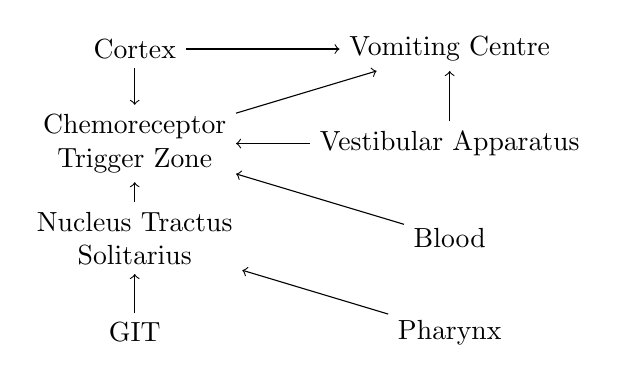
\begin{tikzpicture}

%nodes
\node (1) [word] {Cortex};
\node(2) [word, right of=1, xshift=3cm] {Vomiting Centre};
\node(3) [word, below of=1, yshift = -0.2cm] {Chemoreceptor \\ Trigger Zone};
\node(4) [word, right of=3, xshift=3cm] {Vestibular Apparatus};
\node(5) [word, below of=3, yshift = -0.2cm] {Nucleus Tractus \\ Solitarius};
\node(6) [word, right of=5, xshift=3cm] {Blood};
\node(7) [word, below of=5, yshift = -0.2cm] {GIT};
\node(8) [word, right of=7, xshift=3cm] {Pharynx};

%arrows

\draw [->] (1) -- (2);
\draw [->] (1) -- (3);
\draw [->] (4) -- (3);
\draw [->] (3) -- (2);
\draw [->] (4) -- (2);
\draw [->] (5) -- (3);
\draw [->] (6) -- (3);
\draw [->] (7) -- (5);
\draw [->] (8) -- (5);

\end{tikzpicture}
\end{document}